The methodology described in Chapter \ref{chap:rom} will initially be applied to three relatively simple problems in reactor physics, each building on its predecessors in complexity. The purpose of the simple problems is to develop some untuition about the workings of the described reduced order model algorithm. Ultimately, the methods will be applied to solve a state of the art problem in reactor uncertainty quantification and sensitivity analysis.

% Infinite Assembly
\section{Infinite Lattice Multiplication Factor}
\label{sec:infinite_lattice}

\subsection{Problem Statement}
\label{subsec:infinite_lattice_ps}

In an infinite lattice a reactor of infinite size is considered and therefore neutrons are not capable of leaking out of the system. An infinite lattice effectively removes the effects of geometry in neutron transport and characterizes the system entirely in terms of its material properties. Since the physics of an infinite lattice are greatly simplified an analytic analysis of the system is possible. Consequently, the infinite lattice problem is ideal for an initial analysis of any new computational method. 

To begin, the mathematical formulation of an infinite lattice will be described. In matrix form the two-group neutron balance equations for an infinite lattice can be written as,
\begin{equation}
\label{eq:infinite_lattice_neutron_balance}
   \left(
    \begin{array}{cc}
     \Sigma_{a_1} + \Sigma_{1\rightarrow 2} & 0 \\
     -\Sigma_{12} & \Sigma_{a_2} 
    \end{array}
   \right)
   \left(
    \begin{array}{c}
     \phi_1 \\
     \phi_2
    \end{array}
   \right) 
   = \frac{1}{k_{\infty}}
   \left(
    \begin{array}{cc}
     \nu\Sigma_{f_1} & \nu\Sigma_{f_2} \\
     0 & 0 
    \end{array}
   \right)
   \left(
    \begin{array}{c}
     \phi_1 \\
     \phi_2
    \end{array}
   \right). 
\end{equation}  
Solving the system in \ref{eq:infinite_lattice_neutron_balance} for the infinite multiplication factor, the following analytic expression is obtained,
\begin{equation}
\label{eq:infinite_lattice_kinf}
   k = \frac{\Sigma_{a_2}\nu\Sigma_{f_1} + 
             \Sigma_{1\rightarrow 2}\nu\Sigma_{f_2}}{
              \Sigma_{a_2}\left(
               \Sigma_{a_1} + \Sigma_{1\rightarrow 2}\right)}.
\end{equation}
The infinite multiplication factor is a function of five material parameters. Since this thesis is concerned with the affect of uncertainties in input parameters on computer code outputs, variations in $k_{\infty}$ as a function its stochastic input variables are of interest. Assume all variation in $k_{\infty}$ can be attributed to its input cross sections, whose distributions follow a multivariate Gaussian. To obtain physical homogenized, two-group cross section values a real system must first be modeled in a transport code. The \ac{UAM} Benchmark is sought for this purpose \cite{UAM_Benchmark}. Specifically, the \ac{TMI} assembly is modeled using the two-step method described in \cite{TwoStep_Approach}. A total of 300 perturbed cross section sets were produced to obtain the few-group mean and covariance data used in the proceeding analysis. The cross section data is summarized in Table \ref{table:infintie_lattice_tmi_data}.      
\begin{table}[!htb]
\caption[TMI infinite lattice two-group cross sections.]{\label{table:infintie_lattice_tmi_data} 
Two-group cross section data for an infinite TMI lattice.}
\centering
\begin{tabular}{||c||c|c|c|c|c|c|c||} 
\hline \hline
  &  &  & \multicolumn{5}{|c||}{\textbf{Correlation Coefficient Matrix}}  \\ \hline
  & \textbf{Mean} & \textbf{Standard Dev.} & $\Sigma_{a_1}$ & $\Sigma_{a_2}$ & 
  $\nu\Sigma_{f_1}$ & $\nu\Sigma_{f_2}$ & $\Sigma_{1\rightarrow 2}$ \\ \hline \hline
$\Sigma_{a_1}$ & 1.04E-02 & 9.06E-05 & 1 & 0.07 & -0.13 & 0.02 & 0.75 \\ \hline
$\Sigma_{a_2}$ & 1.10E-01 & 2.31E-04 & 0.07  &  1     & 0.06  & 0.31 & -0.07 \\ \hline
$\nu\Sigma_{f_1}$ & 9.00E-03 & 4.85E-05 & -0.13 &  0.06  & 1     & 0.33 & -0.10 \\ \hline
$\nu\Sigma_{f_2}$ & 1.91E-01 & 8.87E-04 & 0.02  &  0.31  & 0.33  & 1    & 0.01 \\ \hline
$\Sigma_{1\rightarrow 2}$ & 1.80E-02 & 2.18E-04 & 0.75  &  -0.07 & -0.10 & 0.01 & 1 \\ \hline \hline
\end{tabular}
\end{table}

Multiple methods will be applied to obtain basic statistical and sensitivity data on the infinite multiplication factor. Of course, Monte Carlo sampling using the input cross sections' covariance matrix and applying \ref{eq:sample_covariance} will provide the mean and variance of $k_{\infty}$. Another approach to get at the variance of $k_{\infty}$ is through the "Sandwich Equation"\cite{Jessee_Turinsky},
\begin{equation}
\label{eq:sandwich}
   \sigma^2(k_{\infty}) = S^TCS
\end{equation}      
where $C$ is the covariance matrix for the input data. In equation \ref{eq:sandwich} the array $S$ contains sensitivities of the output to the input parameters. For this problem the vector $S$ contains,
\begin{equation}
\label{eq:sensitivity_vector}
   S^T = \left(
    \begin{array}{ccccc}
     \frac{\partial k_{\infty}}{\partial\Sigma_{a_1}} &
     \frac{\partial k_{\infty}}{\partial\Sigma_{a_2}} &
     \frac{\partial k_{\infty}}{\partial\nu\Sigma_{f_1}} &
     \frac{\partial k_{\infty}}{\partial\nu\Sigma_{f_2}} &
     \frac{\partial k_{\infty}}{\partial\Sigma_{1\rightarrow 2}}
    \end{array}
         \right).
\end{equation} 
Since there exists an analytic expression for $k_{\infty}$ the sensitivity vector for this problem in \ref{eq:sensitivity_vector} is exact. As a side-check the sensitivity vector $S$ can also be constructed using central differencing. The sensitivity of $k_{\infty}$ to the $i^{\text{th}}$ cross section $\Sigma_i$ using central differencing is expressed as, 
\begin{equation}
\label{eq:central_diff_kinf}
   \frac{\partial k_{\infty}}{\partial \Sigma_i}\biggr\rvert_
   {\Sigma_{j\neq i} = \bar{\Sigma}_j}
    \approx \frac{k_{\infty}(\Sigma_i + \Delta\Sigma_i) - 
    k_{\infty}(\Sigma_i - \Delta\Sigma_i)}
    {2\Delta\Sigma_i}
\end{equation} 
where all cross sections $\Sigma_j$, $j\neq i$, are held at their mean values. Generally a one percent perturbation $\Delta\Sigma$ is sufficient to obtain accurate sensitivities although this rule of thumb is dependent on the smoothness of the objective function. With a variety of methods available to obtain sensitivities and statistical moments of $k_{\infty}$ it is possible to thoroughly assess the potential of a reduced order model.       
     
\subsection{Analysis}
\label{subsec:kinf_analysis}

Several elements of the methodologies described in Chapter \ref{chap:rom} will be tested in this section and compared to results obtained using analytic and Monte Carlo approaches. For all Smolyak sparse grids constructed the hypercube domain extends to six standard deviations in each random variable. Since $k_{\infty}$ is a function of only five random variables a sparse grid interpolant will be constructed without applying any function decomposition in order to demonstrate the accuracy and convergence of the method. The convergence criteria for the sparse grid interpolant is set such that the maximum hierarchical surplus at a given level is not to exceed $10^{-10}$. Both Clenshaw-Curtis and Gauss-Patterson abscissas are tested. 
\begin{figure}
\caption[Hierarchical surplus convergence for infinite TMI lattice.]{ \label{fig:kinf_sg_convergence}
Convergence study of a five dimensional sparse grid interpolant for the  multiplication factor of an infinite TMI lattice. The boxed numbers represent the current number of knots in the sparse grid.}
 \begin{center}
  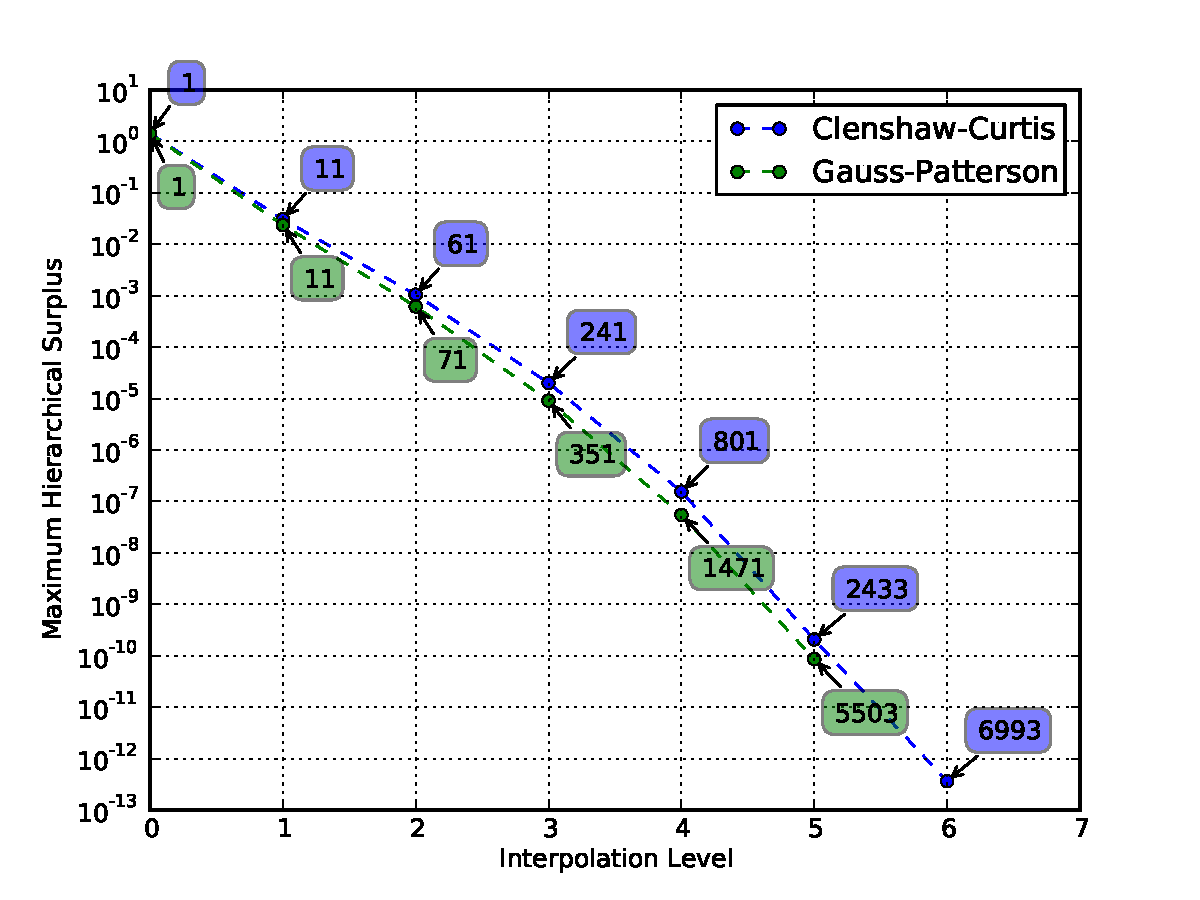
\includegraphics[scale=.75]{./Chapter3/kinf_sparse_grid_convergence.pdf}
 \end{center}
\end{figure}

From Fig. \ref{fig:kinf_sg_convergence} the Clenshaw-Curtis and Gauss-Patterson schemes perform similarly in terms of level to level convergence. However, observe that at each interpolation level the Gauss-Patterson scheme requires significantly more nodes in exchange for a small increase in convergence speed. Both schemes converge to the threshold around level five although the Gauss-Patterson scheme requires more than twice as many function evaluations to get there than Clenshaw-Curtis. Based on the graphical determination of order of convergence \cite{Boyd}, it is clear from \ref{fig:kinf_sg_convergence} that the Smolyak interpolant for $k_{\infty}$ converges geometrically.

With the Smolyak interpolation routines working as expected it's safe to apply them to an anchored-\ac{ANOVA} decomposition of $k_{\infty}$. To start, only the first order components will be built and analyzed. The first order components are relatively cheap to produce and often collectively produce very accurate reduced order models \cite{AHSGC_HighDimensions}. Afterwards, all higher order components will be added in order to show that the full anchored-\ac{ANOVA} decomposition can fully reproduce the objective function. Since $k_{\infty}$ is a function of only five random variables there is no point in adaptively constructing the reduced order model as described in Section \ref{subsec:dimension_truncation}.        

As a first comparison between all the models developed for quantifying the uncertainty in $k_{\infty}$ the mean and variance values of each model will be compared. With the exception of the variance obtained using the Sandwich Equation, each model's variance was obtained by propagating 1000 samples of Eq. $\ref{eq:sample_covariance}$ through the model. All samples produced for each model were seeded identically and so the same random numbers were drawn. The mean and variance results, along with 99\% confidence intervals, are summarized in Table \ref{table:kinf_mean_variance}. 
    
\begin{table} 
\caption[Mean and variance for TMI infinite multiplication factor.]{\label{table:kinf_mean_variance} 
Mean and variance data for the multiplication factor of an infinite TMI lattice obtained using Monte Carlo sampling. Wherever sampling was utilized the same random numbers were used.}
\centering
\small
\begin{tabular}{||c|c|c|c|c||} 
\hline \hline
\textbf{Method} & \textbf{Mean} & \textbf{99\% CI} & \textbf{Standard Dev.} & \textbf{99\% CI} \\ \hline
5D Sparse Grid CC      & 1.41562 & (1.41512, 1.41612) & 0.006168 & (0.005909, 0.006544) \\ \hline
5D Sparse Grid GP      & 1.41562 & (1.41512, 1.41612) & 0.006168 & (0.005831, 0.006544) \\ \hline
1D ANOVA CC  & 1.41560 & (1.41510, 1.41610) & 0.006168 & (0.005831, 0.006544) \\ \hline
All ANOVA CC & 1.41562 & (1.41512, 1.41612) & 0.006168 & (0.005831, 0.006544) \\ \hline
1D ANOVA GP  & 1.41560 & (1.41510, 1.41610) & 0.006168 & (0.005831, 0.006544) \\ \hline
All ANOVA GP & 1.41562 & (1.41512, 1.41612) & 0.006168 & (0.005831, 0.006544) \\ \hline
True Function & 1.41562 & (1.41512, 1.41612) & 0.006168 & (0.005831, 0.006544) \\ \hline
Sandwich               &         &                    & 0.006540 &                      \\
\hline \hline
\end{tabular}
\end{table}

The five dimensional sparse grid interpolant results are entirely self consistent with the anchored-\ac{ANOVA} results. Further, both of these methods produce identical results to those obtained using Monte Carlo sampling. Although the analytic variance from the Sandwich Equation is within the 99\% confidence bounds of each model's results, there is a notable difference due to the fact that only 1000 samples were used to obtain each model's statistics. Increasing the number of samples decreased the difference. Note that in Table \ref{table:kinf_mean_variance} the anchored-\ac{ANOVA} the reduced order models consisting of only one dimension anchored-\ac{ANOVA} components perform just as well as the full decomposition and the sparse grid interpolants over all five random variables. However, the 1D component models require only 29 function evaluations to produce, which is some ten times fewer evaluations than the 5D interpolants, and some hundred times fewer evaluations than the full decomposition. 
\begin{figure}
\caption[Cumulative knot count for constructing an anchored-\ac{ANOVA} decomposition.]{ \label{fig:kinf_numknots}
Cumulative number of knots required at each level of an anchored-\ac{ANOVA} decomposition of the multiplication factor of an infinite TMI lattice. Boxes contain the calculated standard deviation at the current level.}
 \begin{center}
  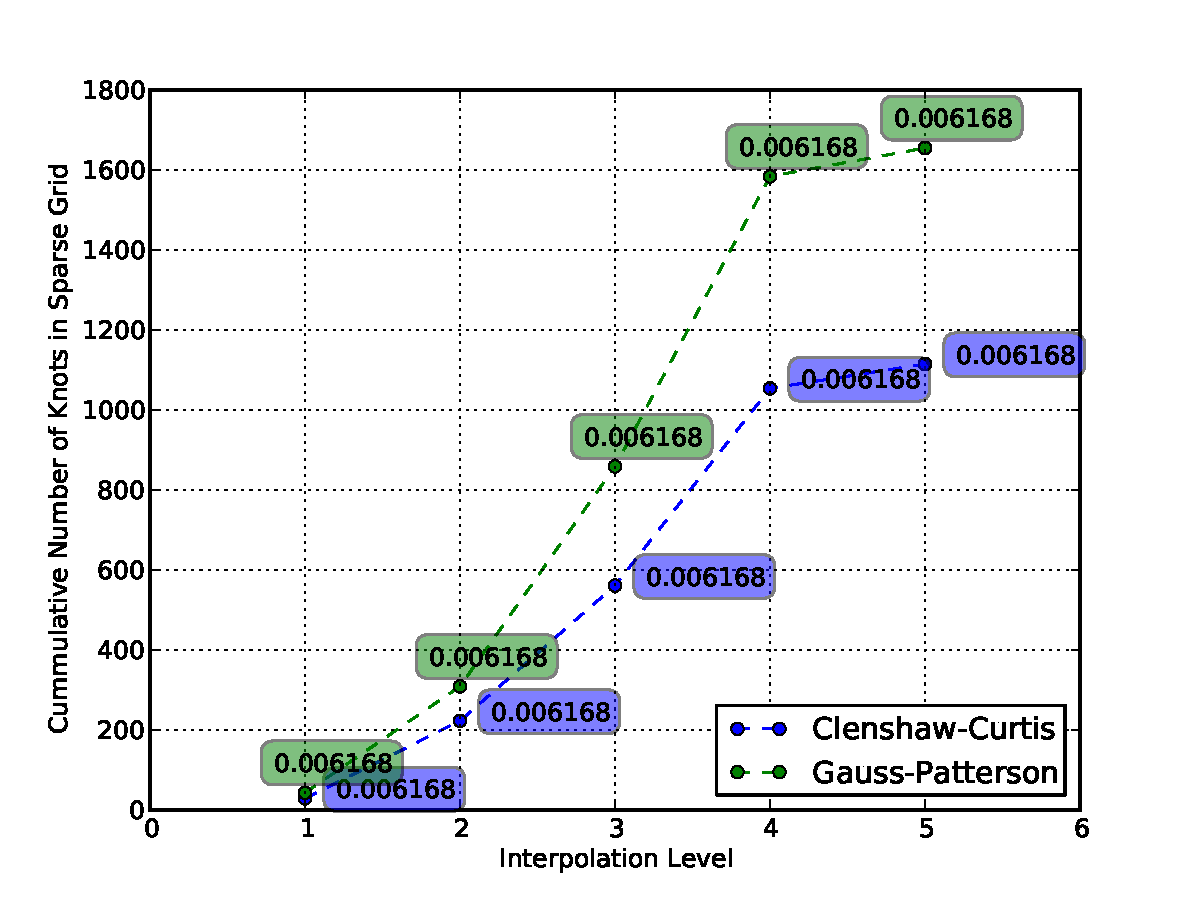
\includegraphics[scale=.75]{./Chapter3/kinf_sparse_grid_numknots.pdf}
 \end{center}
\end{figure}
The rapid convergence of the reduced order model containing only one dimensional anchored-\ac{ANOVA} components is shown in \ref{fig:kinf_numknots}. Construction of higher order components is very expensive. Fortunately for this problem, and perhaps others, construction of only one dimensional components is completely sufficient to represent the objective function. 

As another performance measure of the reduced order model methodologies, each model is used to obtain normalized sensitivity coefficients for $k_{\infty}$. Central differencing is applied to each model, with perturbations made to each cross section at a time while holding the other cross sections at their mean values. Perturbations are taken to be 1\% of each cross section's value. Using the analytic expression for $k_{\infty}$ in \ref{eq:infinite_lattice_kinf}, the central differencing results can be compared to the true sensitivity coefficients.   The results are summarized in Table \ref{table:kinf_sensitivities}. Table \ref{table:kinf_sensitivities}, sensitivity coefficients are also obtained by applying central differencing to the true function as in Eq. \ref{eq:central_diff_kinf}. 
\begin{table}
\caption{\label{table:kinf_sensitivities} 
Normalized sensitivity coefficients for the multiplication factor of an infinite TMI lattice.}
\centering
\begin{tabular}{||c|c|c|c|c|c||} 
\hline \hline
  & \multicolumn{5}{|c||}{\textbf{Normalized Sensitivity Coefficient of $k_{\infty}$}}  \\ \hline
\textbf{Method} & $\Sigma_{a_1}$ & $\Sigma_{a_2}$ & $\nu\Sigma_{f_1}$ & $\nu\Sigma_{f_2}$ & $\Sigma_{1\rightarrow 2}$ \\ \hline
5D Sparse Grid CC  & -.367551 & -.776087 & .224060 & .776010 & .143491 \\ \hline
5D Sparse Grid GP  & -.367551 & -.776087 & .224060 & .776010 & .143491 \\ \hline
1D ANOVA CC        & -.367556 & -.776098 & .224063 & .776020 & .143493 \\ \hline
All ANOVA CC       & -.367551 & -.776087 & .224060 & .776010 & .143491 \\ \hline
1D ANOVA GP        & -.367556 & -.776098 & .224063 & .776020 & .143493 \\ \hline
All ANOVA GP       & -.367551 & -.776087 & .224060 & .776010 & .143491 \\ \hline
Analytic           & -.367520 & -.775956 & .224044 & .775956 & .143476 \\ \hline
Central Difference & -.367551 & -.776089 & .224060 & .776011 & .143492 \\
\hline \hline
\end{tabular}
\end{table}
As expected, all models utilizing the central differencing formula produce self consistent sensitivity coefficients. The models differ from the analytic sensitivity coefficients only in the fourth decimal place, which is expected given the $\mathcal{O}(\Delta\Sigma^2)$ convergence  of the central differencing formula.

Finally, the performance of a Kriging surrogate, as described in section \ref{sec:kriging}, in modeling the infinite multiplication factor will be assessed. Before a Kriging surrogate is constructed the designer must agree on the number of points that will be used to construct the surrogate. As the number of points increases the accuracy of the Kriging surrogate is expected to increase. Recall that each point requires an evaluation of the true objective function, in this case Eq. \ref{eq:infinite_lattice_kinf}. Since Eq. \ref{eq:infinite_lattice_kinf} is linear relatively few sampling points are expected to exactly reproduce the objective function. Indeed, these expectations are demonstrated in
Fig. \ref{fig:kinf_kriging}.  
\begin{figure}
\caption[Reduction in Kriging surrogate error for infinite multiplication factor with increase in points.]{ \label{fig:kinf_kriging}
Reduction in Kriging surrogate error for the infinite multiplication factor as the number of points used to build the surrogate increases.}
 \begin{center}
  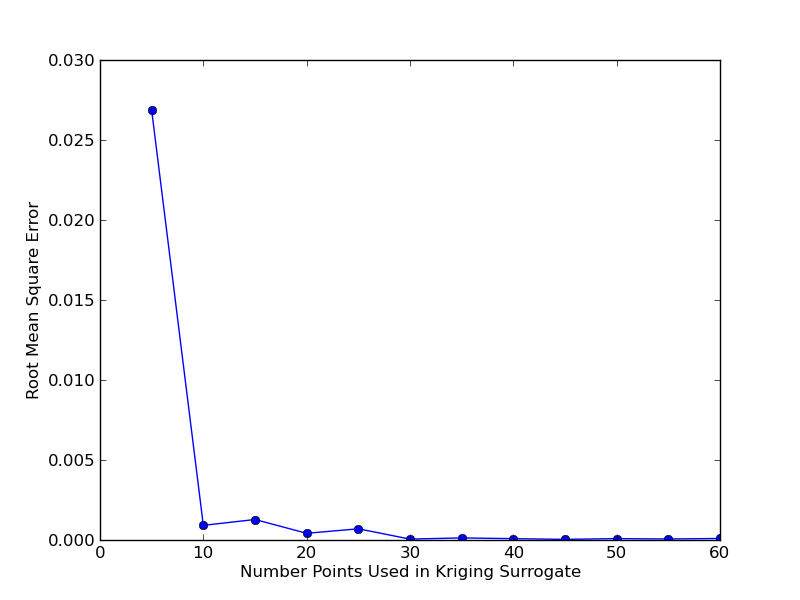
\includegraphics[scale=.75]{./Chapter3/error_vs_npoints.png}
 \end{center}
\end{figure}

In Fig. \ref{fig:kinf_kriging} the number of points used to construct the Kriging surrogate is gradually increased. For each surrogate the root mean square error is calculated by having both Eq. \ref{eq:infinite_lattice_kinf} and the surrogate evaluate the same 100 randomly chosen points in the design space. Observe that for ten evaluation points, which is twice the number of design variables in the objective function, the error essentially goes to zero. This result can be explained by Eq. \ref{eq:infinite_lattice_kinf}'s linearity and the fact that Kriging is an interpolation method, thus requiring a pair of points in each dimension for exact interpolation.     

   

% Kinetics/Thermalhydraulics 
\section{Point Kinetics/Lumped Thermal Hydraulics}
\label{sec:pointkinetics_th}

\subsection{Problem Statement}
\label{subsec:pointkinetics_th_ps}

A reduced order model based on the anchored-\ac{ANOVA} decomposition will be constructed in this section for a simple system of ordinary differential equations modeling a transient in a BN800 sodium fast cooled reactor. The physical model of the reactor consists of point kinetics to model the neutronics and lumped thermal hydraulics equations to describe temperature feedback. The coupled system is nonlinear and only has a time dependence. Previous research groups have utilized point kinetics and lumped thermal hydraulics equations to model basic reactor systems in \cite{Gilli_annals}, \cite{Gilli_mc2011}, and \cite{Housiadas}. In this section a reduced order model will be constructed for the maximum fuel temperature attained following a reactivity insertion as a function of the random variables exhibited in the description of the point kinetics/lumped thermal hydraulics system.  

The six-group point kinetics equations modeling the neutronics of a reactor consist of a balance for reactor power $P(t)$ and a balance equation for each of the six precursor concentrations $C_k(t)$. Changes in reactor power are dependent on the precursor concentration, decays constants $\lambda_k$, delayed neutron fraction $\beta$ and the mean neutron generation time $\Lambda$ as detailed in,
\begin{equation}
\label{eq:pk_power}
   \frac{dP}{dt} = \frac{\rho(T_f,T_c,t)-\beta}{\Lambda}P +
    \sum_{k=1}^6 \lambda_k C_k.
\end{equation}  
The reactivity $\rho$ depends on feedback from the fluids temperature models for the reactor fuel and coolant, which in turn depend on reactor power. The expression for each of the $k$ precursor concentrations is written as,
\begin{equation}
\label{eq:pk_precursors}
   \frac{dC_k}{dt} = -\lambda_k C_k +
    \frac{\beta_k}{\Lambda}P.
\end{equation}
As for the ordinary differential equations describing the behavior of the reactor coolant system, two coupled equations suffice. For the fuel temperature $T_f$, the following lumped model is used,
\begin{equation}
\label{eq:pk_fuel}
   M_f c_{pf}\frac{dT_f}{dt} = P + Ah(T_c-T_f)
\end{equation}
where $M_f$ is the lump fuel mass, $c_{pf}$ is the specific heat capacity of the fuel, $A$ is the heat transfer surface, and $h$ is the heat transfer coefficient between the coolant and reactor fuel. Finally, the coolant temperature is described as,
\begin{equation}
\label{eq:pk_coolant}
   M_c c_{pc}\left(\frac{dT_c}{dt} +v \frac{T_c - T_{in}}{L}\right) = 
    Ah(T_f-T_c)
\end{equation}
where $M_c$ is the lump coolant mass, $c_{pc}$ is the specific heat capacity of the coolant, $L$ is the coolant channel length, $v$ is the coolant flow velocity, and $T_{in}$ is the inlet coolant temperature. The initial conditions for $P$, $C_k$, $T_f$, and $T_c$ depend on the initial power in the reactor $P_0$ before any kind of transient occurs and are listed in \ref{eq:pk_initial_conds}. 
\begin{eqnarray}
\label{eq:pk_initial_conds}
   P(0) &=& P_0 \\ 
   C_k(0) &=& \frac{\beta_k}{\lambda_k\Lambda}P_0 \nonumber \\
   T_f(0) &=& T_c(0) + \frac{P_0}{Ah} \nonumber \\
   T_c(0) &=& T_{in} + \frac{P_0L}{M_c c_{pc}v} \nonumber
\end{eqnarray}
Serving as the coupling device between the lumped thermal hydraulics model and point kinetics model is the reactivity, which is proportional to the coolant temperature and the fuel temperature. Of course, any external reactivity $\rho_{ex}$ added to the reactor is also a contributor. The time dependent reactivity is given explicitly as,
\begin{equation}
\label{eq:pk_reactivity}
   \rho(T_f,T_c,t) = \rho_{ex} + \alpha_d(T_f - T_f(0))
    + \alpha_c(T_c - T_c(0))
\end{equation}
where $\alpha_d$ and $\alpha_c$ are the doppler and coolant coefficients of reactivity, respectively.  

The equations in \ref{eq:pk_power}, \ref{eq:pk_precursors}, \ref{eq:pk_coolant}, and \ref{eq:pk_fuel} are used to model the transient resulting from a half sawtooth external reactivity insertion, as shown in \ref{eq:pk_half_sawtooth}. 
\begin{equation}
\label{eq:pk_half_sawtooth}
   \rho_{ex}(t) = \left\{
    \begin{array}{cr}
     t\rho_{max}/20 & t \leq 20 \\
     0                      & t > 20 
    \end{array}
    \right.
\end{equation}
By treating the coefficients in the point kinetics/lumped thermal hydraulics model as random variables, the objective function investigates the response surface for the maximum fuel temperature attained during transient. The reduced order methodologies will be tested against the stated problem. A depiction of the transient at the random variables' mean values, along with the external reactivity is shown in Figure \ref{fig:pk_transient}.  
\begin{figure}
\caption[Half sawtooth external reactivity insertion transient behavior.]{ \label{fig:pk_transient}
Transient resulting from a half sawtooth external reactivity insertion, as modeled using the mean parameter values of the point kinetics/lumped thermal hydraulics system.}
 \begin{center}
  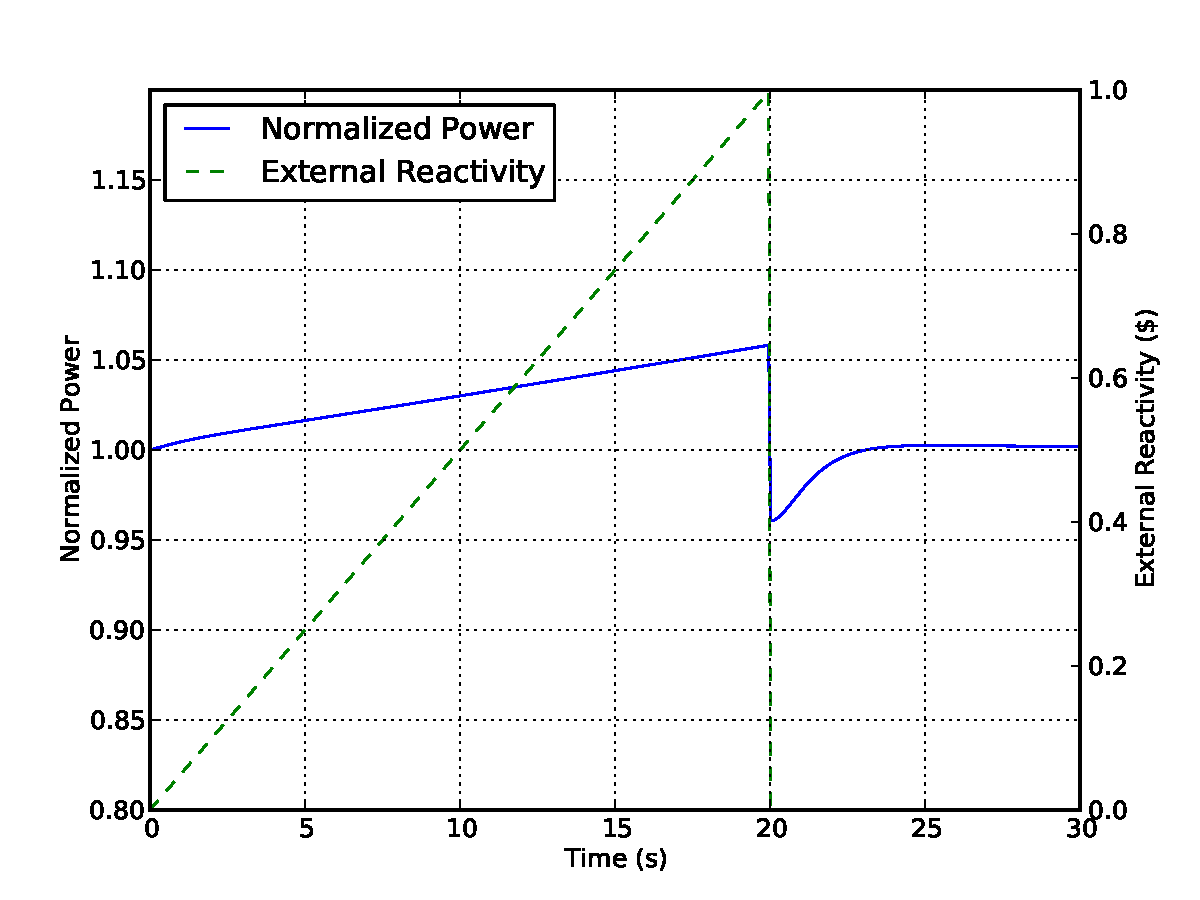
\includegraphics[scale=.75]{./Chapter3/pk_power.pdf}
 \end{center}
\end{figure}
A total of twenty two random variables will be investigated for their affect on the maximum fuel temperature attained during transient. The random variables' mean values, along with their standard deviations are listed in \ref{table:pkinetics_parameters}. Note that all standard deviations are taken to be 5\% of the mean value. All random variables are assumed to be independent of one another, as was assumed in \cite{Gilli_mc2011}. 
\begin{table} 
\caption[Parameter values used in a point kinetics/lumped thermal hydraulics model of a BN800 fast sodium cooled reactor.]{\label{table:pkinetics_parameters} 
Mean parameter values used in the point kinetics/lumped thermal hydraulics model for the analysis of a BN800 fast sodium cooled reactor.}
\centering
\begin{tabular}{||c|c|c|c||} 
\hline \hline
\textbf{Random Variable} & \textbf{Units} & \textbf{Mean} & \textbf{Standard Dev.} \\ \hline
$\lambda_1$  &  $s^{-1}$      &  1.24E-02  &  6.20e-04  \\ \hline
$\lambda_2$  &  $s^{-1}$      &  3.05E-02  &  1.52e-03  \\ \hline
$\lambda_3$  &  $s^{-1}$      &  1.11E-01  &  5.55e-03  \\ \hline
$\lambda_4$  &  $s^{-1}$      &  3.01E-01  &  1.50e-02  \\ \hline
$\lambda_5$  &  $s^{-1}$      &  1.14E+00  &  5.70e-02  \\ \hline
$\lambda_6$  &  $s^{-1}$      &  3.01E+00  &  1.50e-01  \\ \hline
$\beta_1$    &                &  9.00E-05  &  4.50e-06  \\ \hline
$\beta_2$    &                &  8.53E-04  &  4.26e-05  \\ \hline
$\beta_3$    &                &  7.00E-04  &  3.50e-05  \\ \hline
$\beta_4$    &                &  1.40E-03  &  7.00e-05  \\ \hline
$\beta_5$    &                &  6.00E-04  &  3.00e-05  \\ \hline
$\beta_6$    &                &  5.50E-04  &  2.75e-05  \\ \hline
$\Lambda$    &  $s$           &  4.00E-07  &  2.00e-08  \\ \hline
$Ah$         &  $kW/K$        &  2.50E+06  &  1.25e+05  \\ \hline
$M_c$        &  $kg$          &  1.16E+03  &  5.84e+01  \\ \hline
$M_f$        &  $kg$          &  9.67E+03  &  4.83e+02  \\ \hline
$c_{pc}$     &  $J/kg\cdot K$ &  1.20E+03  &  6.00e+01  \\ \hline
$c_{pf}$     &  $J/kg\cdot K$ &  5.00E+02  &  2.50e+01  \\ \hline
$v$          &  $m/s$         &  7.50E+00  &  3.75e-01  \\ \hline
$\alpha_d $  &  $pcm/K$       &  6.87E-06  &  3.43e-07  \\ \hline
$\alpha_c$   &  $pcm/K$       &  1.23E-06  &  6.15e-08  \\ \hline
$\rho_{max}$ &                &  4.19E-04  &  2.09e-05  \\ 
\hline \hline
\end{tabular}
\end{table}
A plot of the fuel temperature as a function of time due to the external reactivity profile shown in the same figure is depicted in Figure \ref{fig:pk_fuel_temp}. 
\begin{figure}[!htb]
\caption[Fuel temperature transient resulting from a half sawtooth reactivity insertion.]{ \label{fig:pk_fuel_temp}
Fuel temperature transient resulting from a half sawtooth reactivity insertion. All parameters in the coupled point kinetics/lumped thermal hydraulics equations are held at their mean values. 
}
 \begin{center}
  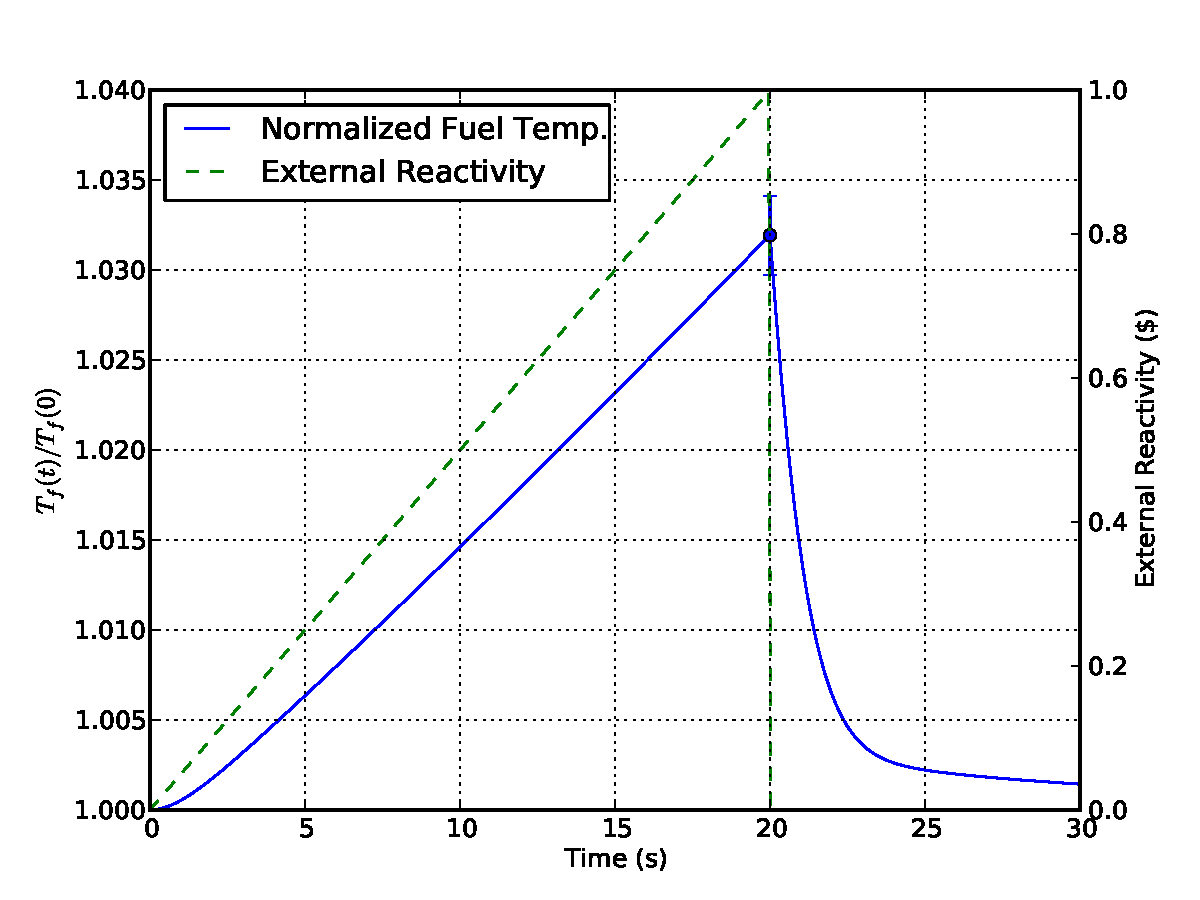
\includegraphics[scale=.75]{./Chapter3/pk_fueltemp.pdf}
 \end{center}
\end{figure}

\subsection{Analysis}
\label{subsec:pointkinetics_th_analysis}

An adaptive reduced order model, whose formulation is summarized in Algorithm \ref{code:rom_algorithm}, will be created for the problem described in section \ref{subsec:pointkinetics_th_ps}. The reduced order model will be investigated for its ability to reproduce statistics of interest by comparing its results with those obtained from sampling the true function. As described in Algorithm \ref{code:rom_algorithm}, the first step in creating a reduced order model for the maximum fuel temperature is to construct all first order components in the anchored-\ac{ANOVA} decomposition and to identify the important ones. The sparse grids comprising the reduced order model are assumed to be converged when the maximum hierarchical surplus for a given level is less than $10^{-5}$. Consequently, at least five digits of accuracy are expected. Important dimensions are those whose normalized sensitivity index in Eq. \ref{eq:anova_sensitivity} exceeds 5\%.

From Figure \ref{fig:pk_importance_pie} the "important" variables are identified to be $Ah$, $\alpha_d$, and $\rho_{max}$. Collectively these three "important" random variables comprise 82\% of the total sensitivity. 
\begin{figure}[!htb]
\caption[Normalized sensitivity indices for random variables comprising the coupled point kinetics/lumped thermal hydraulics equations.]{ \label{fig:pk_importance_pie}
Normalized sensitivity indices for all random variables comprising the coupled point kinetics/lumped thermal hydraulics equations. The effects of all $\beta_k$ and $\lambda_k$ have been lumped into single $\beta$ and $\lambda$ effects, respectively. 
}
 \begin{center}
  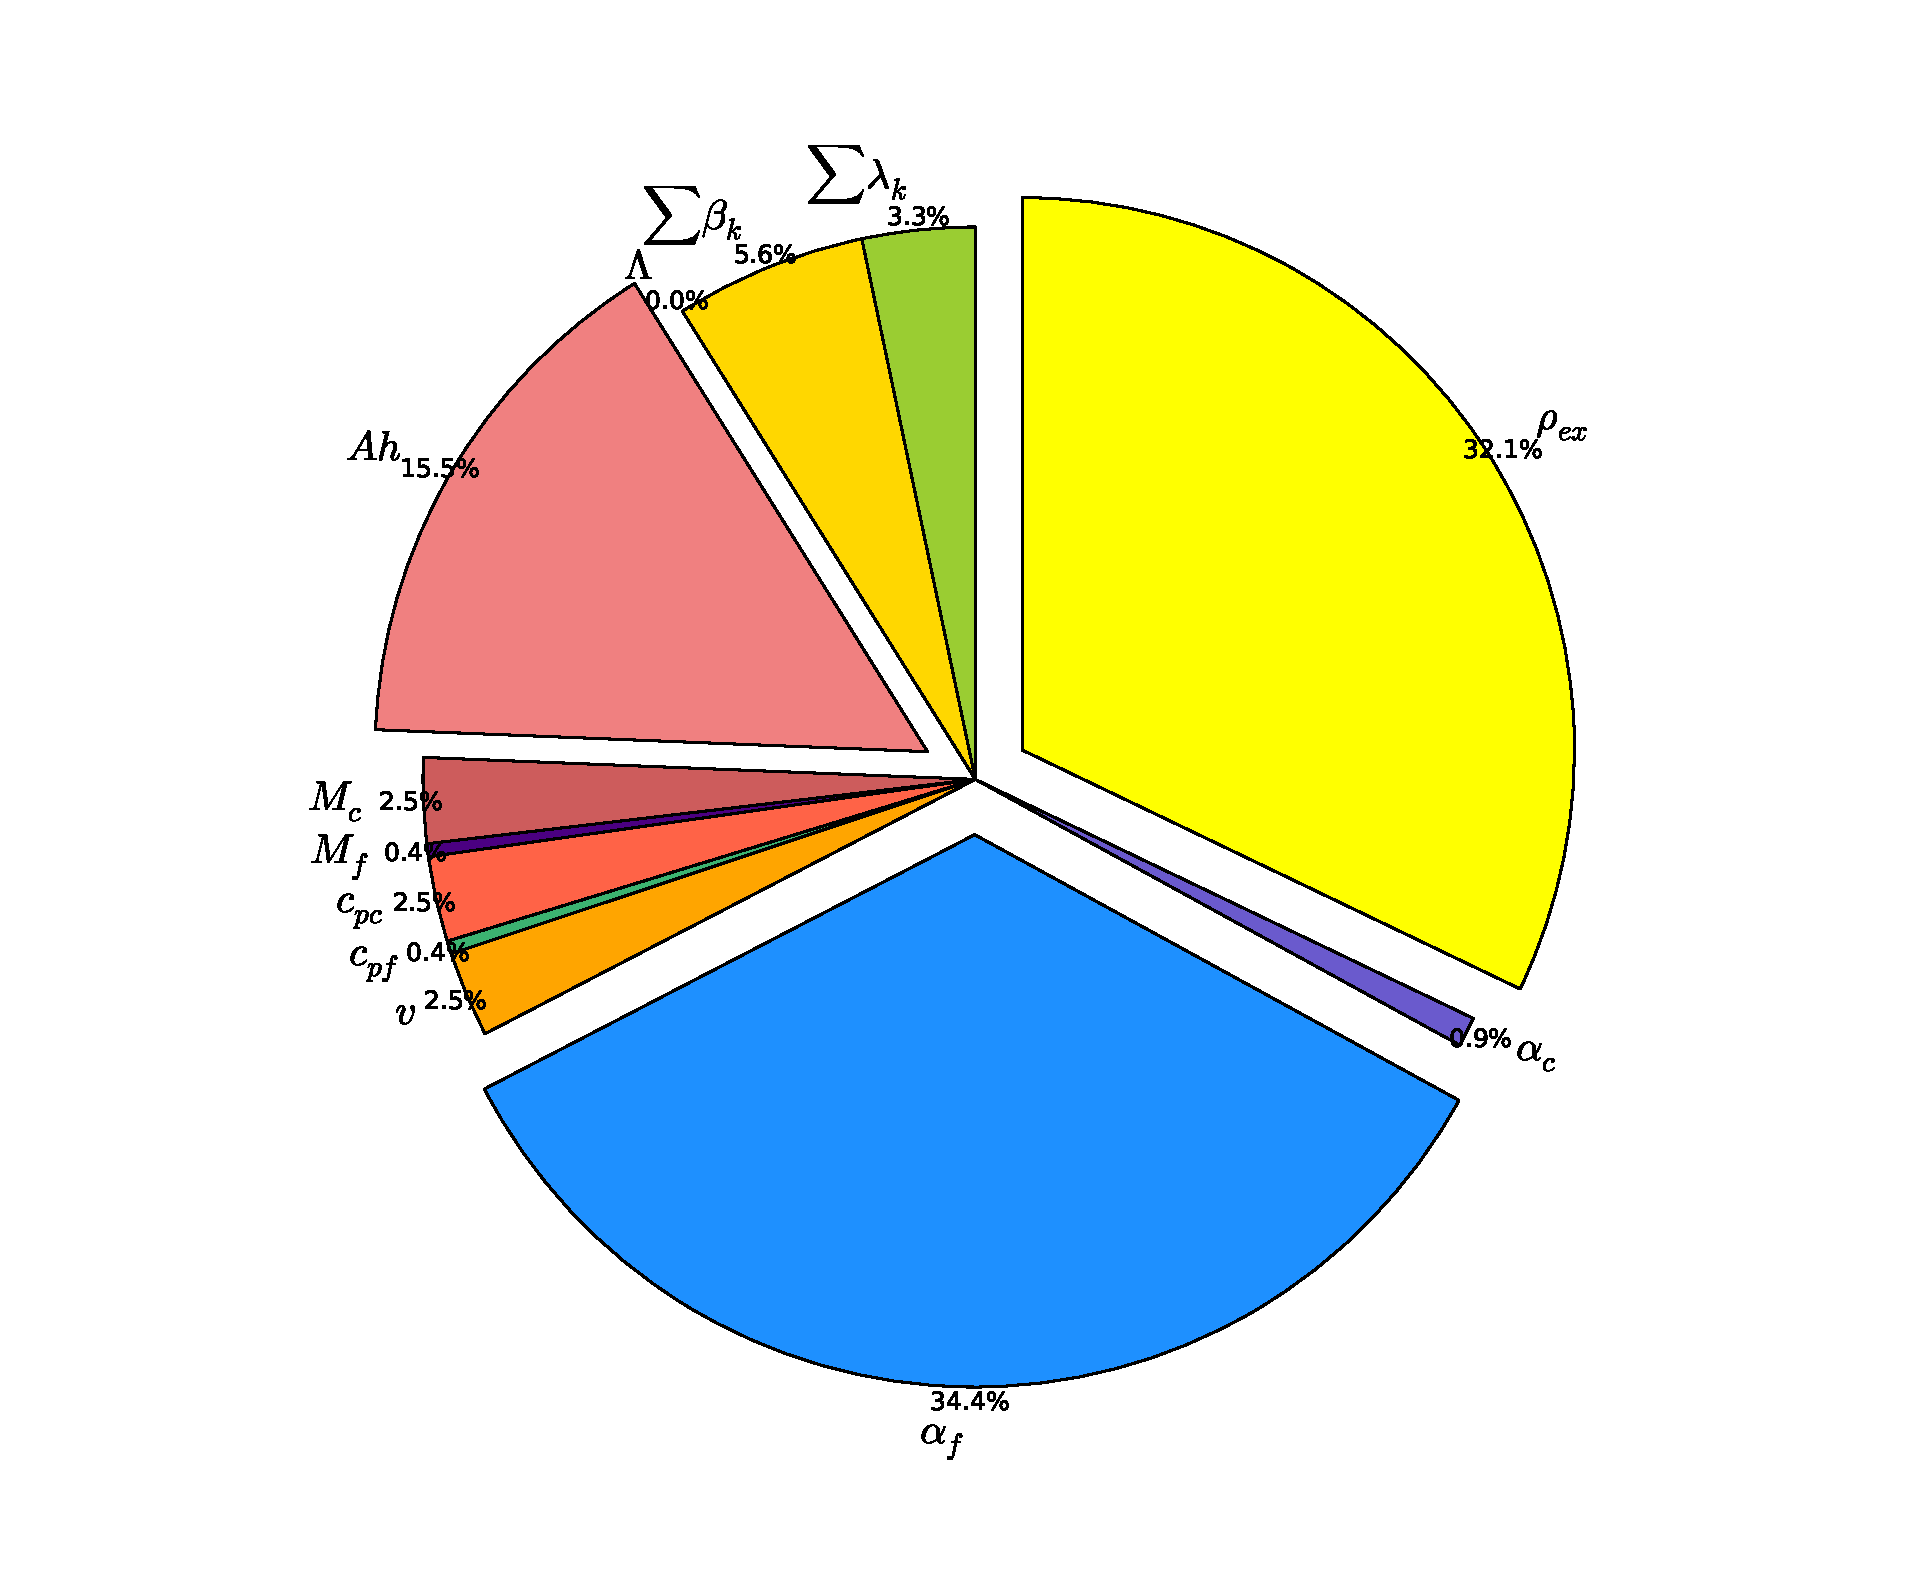
\includegraphics[scale=.5]{./Chapter3/pk_importance_pie.pdf}
 \end{center}
\end{figure}
The indication that the maximum fuel temperature is sensitive to the heat transfer $Ah$ from fuel to coolant is not surprising since in Eq. \ref{eq:pk_fuel} the fuel temperature is directly proportional to $Ah$. Further, the random variables $\rho_{max}$ and $\alpha_d$ determine the slope of the increase in fuel temperature, as seen in Figure \ref{fig:pk_fuel_temp}, and so a strong sensitivity to these random variables is expected. The sensitivity of the maximum fuel temperature to $\alpha_c$ is not as great since the increase in coolant temperature during the transient is significantly smaller than the rise in fuel temperature. Relatively weak sensitivity to $M_f$ and $c_{pf}$ can perhaps be attributed to cancellation of error since these two variables are multiplied together.

With only three random variables deemed as "important" only three second order anchored-\ac{ANOVA} components must be built for the reduced order model. Neglecting any convergence criteria, third order component describing the interaction effects among the three important random variables is also built. A summary of the total number of function evaluations needed to construct the adaptive reduced order model for the maximum fuel temperature is shown in Figure \ref{fig:pk_sparse_grid_numknots}.          
\begin{figure}[!htb]
\caption[Cumulative number of knots for constructing a reduced order model of the maximum fuel temperature in the point kinetics/lumped thermal hydraulics model.]{\label{fig:pk_sparse_grid_numknots}
Number of knots needed to adaptively construct a reduced order model for the maximum fuel temperature in both the Clenshaw-Curtis and Gauss-Patterson schemes. Boxed values state the standard deviation calculated at each level.  
}
 \begin{center}
  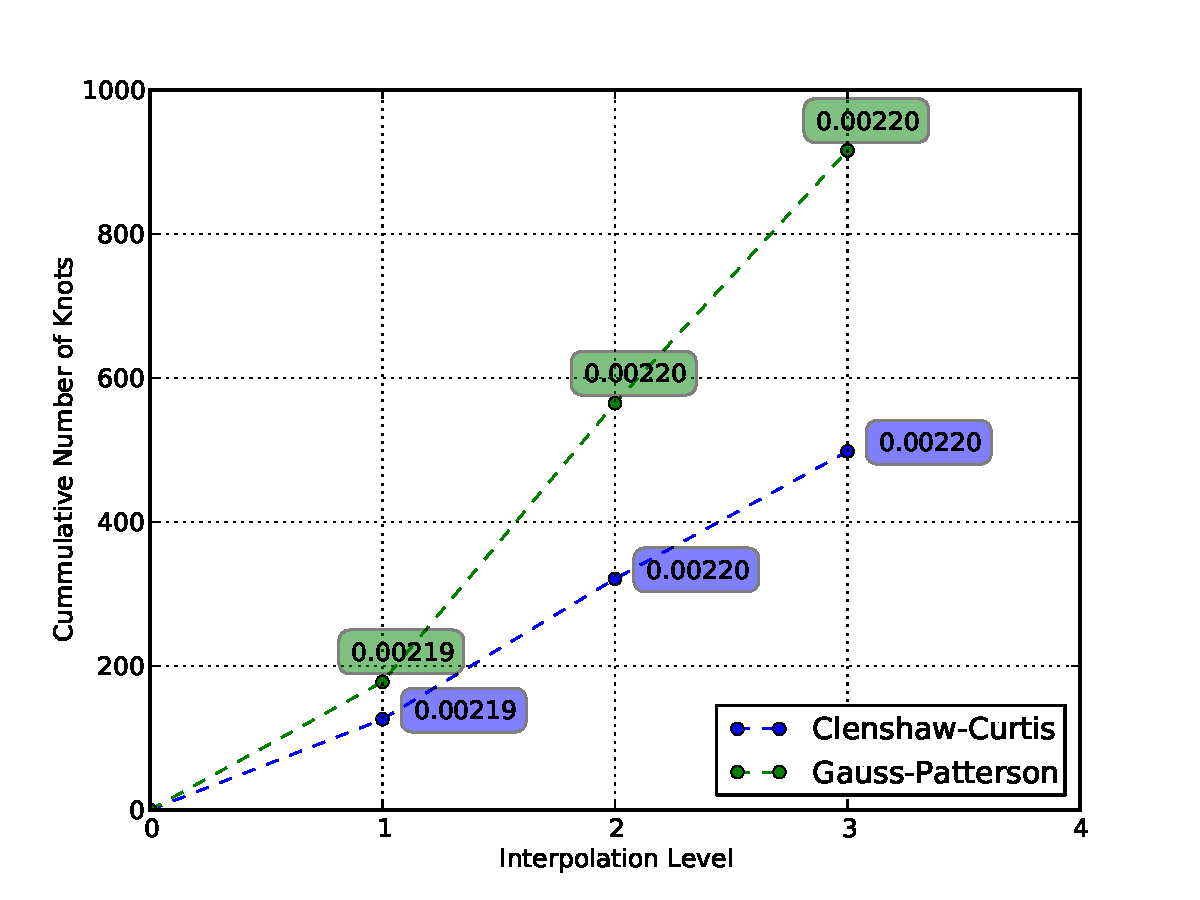
\includegraphics[scale=.75]{./Chapter3/pk_sparse_grid_numknots.pdf}
 \end{center}
\end{figure}
The Gauss-Patterson scheme required almost twice as many knots as Clenshaw-Curtis to adaptively build the reduced order model. From Figure \ref{fig:pk_sparse_grid_numknots} it's clear that the reduced order model consisting of only one dimensional components is effectively just as accurate as the full model, but requiring only 126 function evaluations to build using Clenshaw-Curtis. To see how well the reduced order models are able to reproduce the mean and variance of the true function Monte Carlo simulation is utilized. The models produced using anchored-\ac{ANOVA} decomposition with superposition dimensions of one and three are sampled along with the true function. Mean, variance, and pertinent 99\% confidence intervals for the sampling are summarized in Table \ref{table:pk_mean_variance}. A total of 1000 samples were used for each method, each using the same random numbers.      
\begin{table}[!htb] 
\caption[Mean and variance data for maximum fuel temperature achieved during transient.]{\label{table:pk_mean_variance} 
Mean and variance data for the maximum fuel temperature achieved during transient obtained using Monte Carlo sampling. The same random numbers were used for all 1000 samples for each method.}
\centering
\small
\begin{tabular}{||c|c|c|c|c||} 
\hline \hline
\textbf{Method} & \textbf{Mean} & \textbf{99\% CI} & \textbf{Standard Dev.} & \textbf{99\% CI} \\ \hline
1D ANOVA CC  & 1.03193 & (1.03175, 1.03211) & 0.002187 & (0.002068, 0.002320) \\ \hline
All ANOVA CC & 1.03193 & (1.03175, 1.03211) & 0.002196 & (0.002076, 0.002330) \\ \hline
1D ANOVA GP  & 1.03193 & (1.03175, 1.03211) & 0.002187 & (0.002068, 0.002320) \\ \hline
All ANOVA GP & 1.03193 & (1.03175, 1.03211) & 0.002196 & (0.002076, 0.002330) \\ \hline
True Function & 1.03193 & (1.03175, 1.03211) & 0.002196 & (0.002076, 0.002330) \\ 
\hline \hline
\end{tabular}
\end{table}
As evidenced in Table \ref{table:pk_mean_variance} the statistical results for each method are consistent. While the reduced order model with superposition dimension of three is able to replicate the Monte Carlo results to five significant figures, the expected accuracy, the order-one superposition model is slightly short. Of course, this is due to the absence of higher order components. However, the proximity of the order-one superposition model's results to the true results indicate that for this problem the higher order components do not have a significant impact. To further verify the ability of the reduced order models to accurately reproduce basic statistical moments, the probability distributions for the normalized maximum fuel temperature produced by each model are compared in Figure \ref{fig:pk_histograms}. 
\begin{figure}[!htb]
\caption{\label{fig:pk_histograms}
Histograms produced by sampling the true function, order-one superposition reduced order model, and the full adaptive reduced order model.  
}
 \begin{center}
  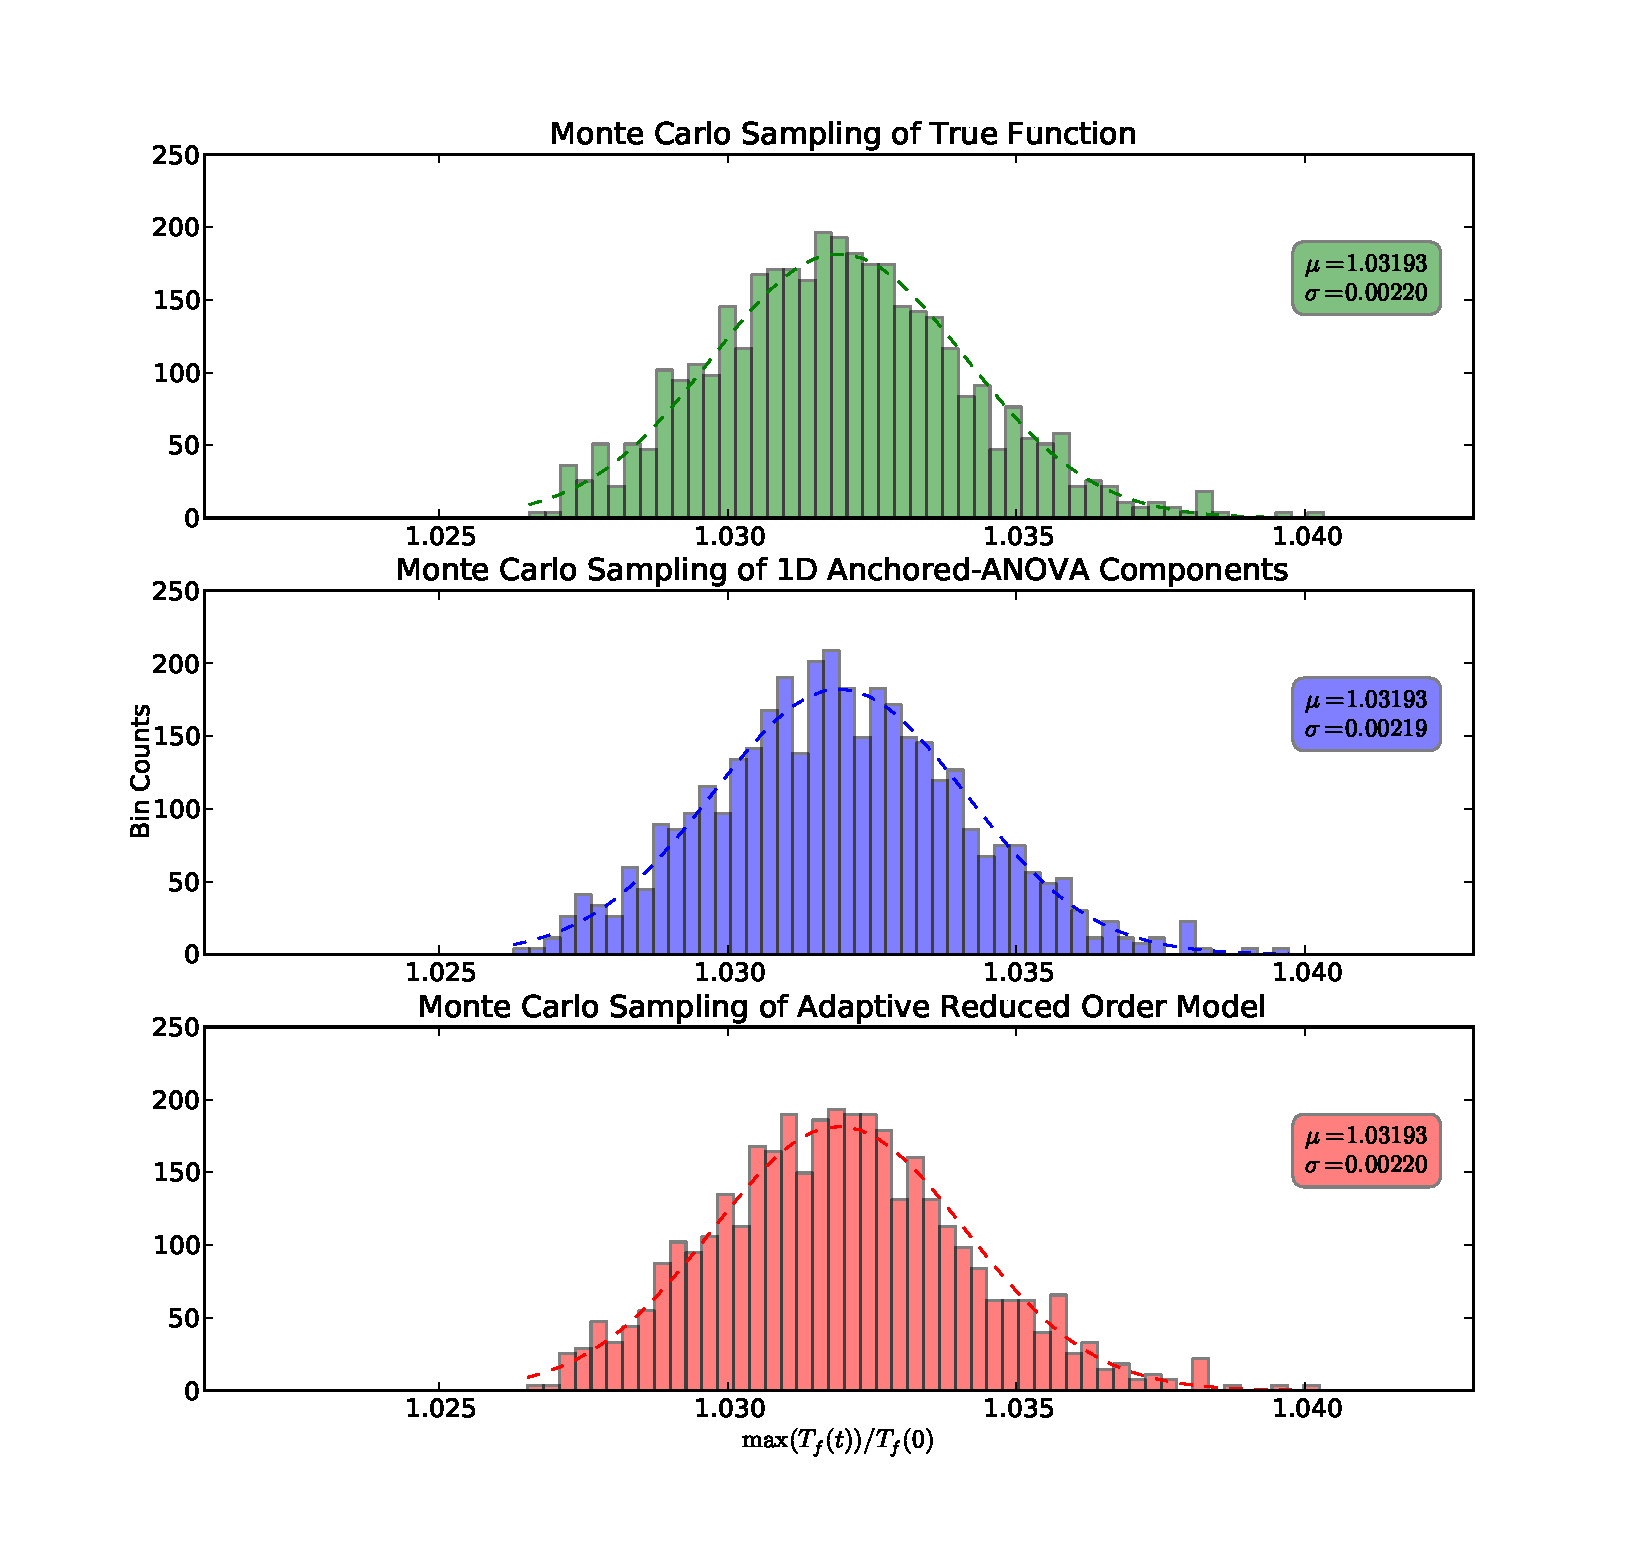
\includegraphics[scale=.58]{./Chapter3/pk_histograms.pdf}
 \end{center}
\end{figure}
All of the tested reduced order models are able to reproduce the Gaussian probability distribution for the normalized maximum fuel temperature. 

As done in section \ref{subsec:kinf_analysis}, a sensitivity analysis will be completed for the reduced order model and compared to the normalized sensitivity coefficients obtained using central differencing. From Table \ref{table:pk_sensitivities} notice that the largest sensitivity coefficients are those of the random variables deemed "important" using the adaptive reduced order model algorithm. Only the sensitivity coefficients for the Clenshaw-Curtis sparse grid are shown in Table \ref{table:pk_sensitivities} since the Gauss-Patterson sparse grid returns identical results. The normalized sensitivity coefficients calculated using the reduced order models are the same as those calculated using central differencing to the expected number of significant digits.   
\begin{table}[!htb] 
\caption{\label{table:pk_sensitivities} 
Normalized sensitivity coefficients of the maximum fuel temperature to random variables.}
\centering
\begin{tabular}{||c|c|c|c||} 
\hline \hline
\textbf{Random Variable} & \textbf{1D ANOVA CC} & \textbf{All ANOVA CC} & \textbf{Central Diff.} \\ \hline
$\lambda_1$  &  3.7894E-05 &  3.7894E-05 &  3.7895E-05 \\ \hline
$\lambda_2$  &  7.0387E-04 &  7.0387E-04 &  7.0387E-04 \\ \hline
$\lambda_3$  &  8.4244E-04 &  8.4244E-04 &  8.4215E-04 \\ \hline
$\lambda_4$  &  9.7308E-04 &  9.7309E-04 &  9.7379E-04 \\ \hline
$\lambda_5$  &  1.1572E-04 &  1.1572E-04 &  1.1607E-04 \\ \hline
$\lambda_6$  &  4.4638E-05 &  4.4639E-05 &  4.0498E-05 \\ \hline
$\beta_1$    & -3.2992E-04 & -3.2992E-04 & -3.2976E-04 \\ \hline
$\beta_2$    & -2.6582E-03 & -2.6582E-03 & -2.6616E-03 \\ \hline
$\beta_3$    & -1.1953E-03 & -1.1953E-03 & -1.2040E-03 \\ \hline
$\beta_4$    & -1.0129E-03 & -1.0129E-03 & -1.0232E-03 \\ \hline
$\beta_5$    & -1.1689E-04 & -1.1689E-04 & -1.1810E-04 \\ \hline
$\beta_6$    & -4.0718E-05 & -4.0718E-05 & -4.1134E-05 \\ \hline
$\Lambda$    & -8.9294E-08 & -8.9295E-08 & -8.9364E-08 \\ \hline
$Ah$         &  1.2553E-02 &  1.2553E-02 &  1.2584E-02 \\ \hline
$M_c$        &  1.8753E-03 &  1.8753E-03 &  1.8716E-03 \\ \hline
$M_f$        & -3.6695E-04 & -3.6695E-04 & -3.6360E-04 \\ \hline
$c_{pc}$     &  1.8753E-03 &  1.8753E-03 &  1.8903E-03 \\ \hline
$c_{pf}$     & -3.6695E-04 & -3.6695E-04 & -3.5976E-04 \\ \hline
$v$          &  1.8838E-03 &  1.8839E-03 &  1.9177E-03 \\ \hline
$\alpha_d $  & -2.6655E-02 & -2.6656E-02 & -2.6625E-02 \\ \hline
$\alpha_c$   &  8.4387E-04 &  8.4387E-04 &  8.7194E-04 \\ \hline
$\rho_{max}$ &  3.1164E-02 &  3.1164E-02 &  3.1272E-02 \\ 
\hline \hline
\end{tabular}
\end{table}

To further analyze the coupled point kinetics/lumped thermal hydraulics problem in hand, Morris' algorithm is applied, as described in section \ref{subsec:morris_algorithm}. As previously described, algorithm \ref{code:morris_algorithm} aims to identify the design variables that have the greatest influence on an objective function's behavior, which in this case is the fuel temperature. To effectively determine such design variables it is convenient to plot the mean against the standard deviation of each design variable's elementary effects. From the problem at hand, the elementary effect statistics are plotted in Fig. \ref{fig:kth_important_vars}.     
\begin{figure}[!htb]
\caption{\label{fig:kth_important_vars}
Statistics of each design variable's elementary effects, as applied to the coupled point kinetics/lumped thermal hydraulics problem.   
}
 \begin{center}
  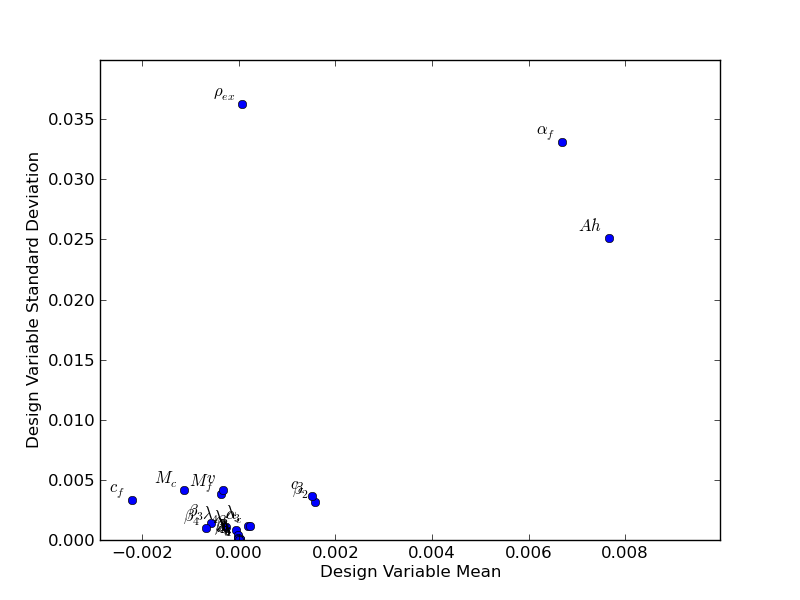
\includegraphics[scale=.75]{./Chapter3/importantvariables.png}
 \end{center}
\end{figure}
Figure \ref{fig:kth_important_vars} was obtained using five divisions and ten elementary effects per design variable. Observe how eighteen of the twenty two points are clustered around the origin, implying that each of these clustered variables have minimal influence on the fuel temperature. In contrast, the variables $\rho_{ex}$, $\alpha_f$, and $Ah$ are likely to be primary contributors. The results of Fig. \ref{fig:kth_important_vars} are entirely consistent with Fig. \ref{fig:pk_importance_pie}, which also identifies the variables $\rho_{ex}$, $\alpha_f$, and $Ah$ as being principally important.      

Now, with the three key variables identified a Kriging surrogate is constructed for the normalized fuel temperature. Sampling the three-dimensional surrogate 1000 times, as done to obtain the results in Table \ref{table:pk_mean_variance}, a mean normalized temperature of $1.03198 \pm 0.002299$ was obtained which is well within the $99\%$ confidence interval of the sampled true result. Note that some of the statistical discrepancies being observed can be attributed to the fact that the same random number were not used in the evaluation of the surrogate and true function. 


% TMI Minicore
\section{\ac{TMI} Minicore}
\label{sec:tmi_minicore}

\subsection{Problem Statement}
\label{subsec:tmi_minicore_ps}

The previous two problems dealt with relatively simple functions that don't require industrial engineering codes to solve. However, the main intention of this thesis is to construct reduced order models for computer codes that aim to model large and complex engineering systems. Interaction with such computer codes consist of input and output files; the governing equations and their solvers are rarely seen. The primary purpose of this demonstration problem is to show that the same algorithms applied to analyze the previous problems are also functional when applied to engineering computer codes.

In this demonstration problem the reactor core simulator code \ac{PARCS} \cite{PARCS} is applied to the \ac{TMI} minicore described in the first phase of the \ac{UAM} Benchmark \cite{UAM_Benchmark}. The minicore problem consists of a three-by-three fuel assembly configuration with reflector blocks placed around the assemblies, as seen in Figure \ref{fig:tmi_minicore}. In the minicore the central assembly is rodded while the periphery fuel assemblies are unrodded. Vacuum boundary conditions are applied. The few-group, homogenized cross section description for each fuel assembly consists of transport, absorption, nu-fission, and scatter cross sections along with values for \ac{ADFs}. For a two-group problem the total number of cross sections to describe an assembly is nine. Since the homogenized reflector region does not support fission only seven homogenized cross sections are required to describe it. Consequently, to model the minicore configuration in Fig. \ref{fig:tmi_minicore} in \ac{PARCS} a total of twenty five homogenzied, two-group cross sections are needed.  
\begin{figure}[!htb]
\caption{\label{fig:tmi_minicore}
\ac{TMI} minicore configuration used for analysis, as defined in the \ac{UAM} Benchmark specifications.}
 \begin{center}
  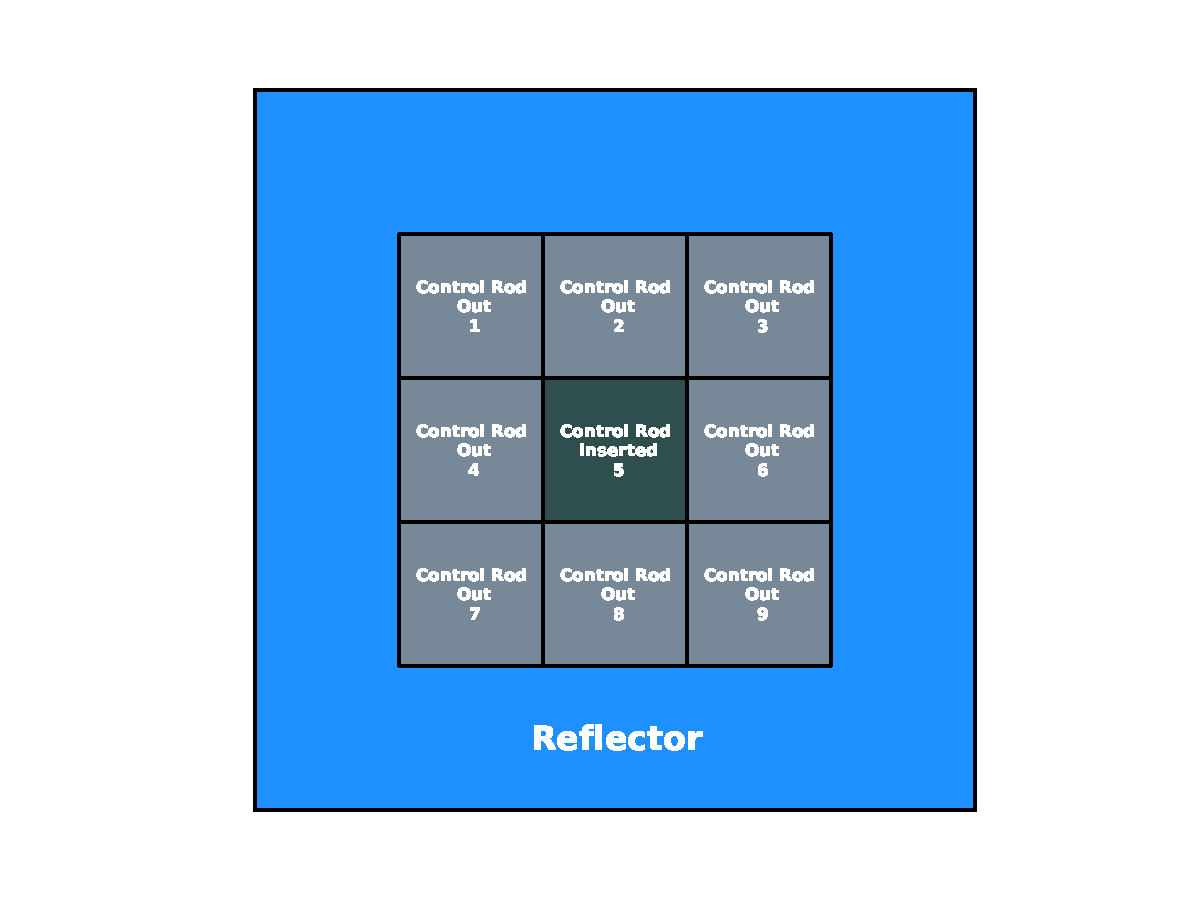
\includegraphics[scale=.75]{./Chapter3/tmi_minicore.pdf}
 \end{center}
\end{figure}  

In order to study the effects of the uncertainties inherent in the few-group cross sections on output parameters of interest in \ac{PARCS}, a few-group covariance matrix is necessary. The few-group covariance matrix is obtained using the 'two-step' method depicted in Fig. \ref{fig:sampler_flow_diagram}. A total of 300 transport calculations with perturbed multigroup cross sections were executed to generate the few-group covariance matrix. In the previous example problems only one output parameter was investigated at a time. However, recall in the discussion of the Smolyak algorithm that interpolation is only performed on the random space. The objective function is evaluated at each abscissa in the random space, returning an output that can still be a function of physical space. In this case the hierarchical surplus is no longer one dimensional. Rather, the hierarchical surplus in Eq. \ref{eq:hierarchical_surplus} is rewritten as,
\begin{equation} 
\label{eq:hierarchical_surplus_space}
   f(\mathbf{x}, x_{j_1}^{i_1},...,x_{j_d}^{i_d}) - 
    A(q-1,d)(\mathbf{x}, x_{j_1}^{i_1},...,x_{j_d}^{i_d})
\end{equation}
where $\mathbf{x} \in \mathcal{D}$ is a coordinate in the spatial domain. When the objective function is a function of spatial coordinates the Smolyak algorithm approximates the function as a linear combination of vectors, the linear weights still being tensor products of basis functions for the random space. To determine the mean and variance of a reduced order model approximation of some space-dependent objective function the $L_2$ norm is taken over the spatial domain $\mathcal{D}$. Similarly, to identify important dimensions using the sensitivity coefficient defined in Eq. \ref{eq:anova_sensitivity} the $L_2$ norm is taken of $\eta_i(\mathbf{x})$.  

The problem in this section considers the core box power distribution of the minicore in Fig. \ref{fig:tmi_minicore} and consequently, the objective function is space dependent. For each simulation in \ac{PARCS} a vector of length nine is returned with each entry containing the relative box power in the fuel assemblies. The box powers are calculated such that the average of all nine entries is identically equal to unity. In the \ac{PARCS} output file the box powers are only given to four digits of accuracy and therefore roundoff error in this problem warrants some attention.  

\subsection{Analysis}
\label{subsec:tmi_analysis}

In this analysis a pure 'two-step' approach is used to compare the results obtained using a reduced order model for the box powers output in \ac{PARCS}. For the 'two-step' approach a few group covariance matrix is constructed and sampled 500 times, with each sample containing perturbed few group cross sections. Each cross section set is propagated through the \ac{PARCS} code and the box powers for the fuel assemblies are extracted from the output file. Ultimately, 500 box power outputs are analyzed statistically to obtain correlations, means, and variances. The same few group covariance matrix is used to sample the reduced order model for the box powers.    

To build a reduced order model, Algorithm \ref{code:rom_algorithm} is applied with a hierarchical surplus threshold of $10^{-4}$ since the \ac{PARCS} box powers are only output to four decimal places. Consequently, roundoff error may accumulate in the fourth decimal point of the reduced order model. A total of 123 executions of \ac{PARCS} were required to construct all single order components of the reduced order model using Clenshaw-Curtis abscissas. Due to the geometry of the \ac{TMI} minicore, 1/8 symmetry is expected in the box power results. Consequently, only fuel assemblies one, four and five are investigated, as defined in Fig. \ref{fig:tmi_minicore}. Sampling results for the mean and standard deviation for the true box power \ac{PARCS} model and the reduced order model are summarized in Tables \ref{table:tmi_mean_sd_mc} and \ref{table:tmi_mean_sd_1d}, respectively. 
%
\begin{table}[!htb] 
\caption{\label{table:tmi_mean_sd_mc} 
Mean and standard deviation data for \ac{TMI} minicore box powers where \ac{PARCS} code is used as objective function. A total of 500 samples were used. Assembly numbers correspond to Fig. \ref{fig:tmi_minicore}.}
\centering
\begin{tabular}{||c|c|c|c|c||} 
\hline \hline
\textbf{Assembly} & \textbf{Mean} & \textbf{99\% CI} & \textbf{Standard Dev.} & \textbf{99\% CI} \\ \hline
1 & 0.8387 & (0.8386, 0.8388) & 0.0007 & (0.0006, 0.0008) \\ \hline 
2 & 1.1499 & (1.1498, 1.1500) & 0.0011 & (0.0010, 0.0012) \\ \hline
3 & 0.8387 & (0.8386, 0.8388) & 0.0007 & (0.0006, 0.0008) \\ \hline
4 & 1.1499 & (1.1498, 1.1500) & 0.0011 & (0.0010, 0.0012) \\ \hline
5 & 1.0453 & (1.0450, 1.0456) & 0.0027 & (0.0025, 0.0029) \\ \hline
6 & 1.1499 & (1.1498, 1.1500) & 0.0011 & (0.0010, 0.0012) \\ \hline
7 & 0.8387 & (0.8386, 0.8388) & 0.0007 & (0.0006, 0.0008) \\ \hline
8 & 1.1499 & (1.1498, 1.1500) & 0.0011 & (0.0010, 0.0012) \\ \hline
9 & 0.8387 & (0.8386, 0.8388) & 0.0007 & (0.0006, 0.0008) \\ 
\hline \hline
\end{tabular}
\end{table}
%
\begin{table}[!htb] 
\caption{\label{table:tmi_mean_sd_1d} 
Mean and standard deviation data for \ac{TMI} minicore box powers where the objective function is a reduced order model for \ac{PARCS} containing only 1D components. A total of 500 samples were used. Assembly numbers correspond to Fig. \ref{fig:tmi_minicore}.}
\centering
\begin{tabular}{||c|c|c|c|c||} 
\hline \hline
\textbf{Assembly} & \textbf{Mean} & \textbf{99\% CI} & \textbf{Standard Dev.} & \textbf{99\% CI} \\ \hline
1 & 0.8387 & (0.8386, 0.8388) & 0.0007 & (0.0006, 0.0008) \\ \hline 
2 & 1.1500 & (1.1499, 1.1501) & 0.0012 & (0.0011, 0.0013) \\ \hline
3 & 0.8387 & (0.8386, 0.8388) & 0.0007 & (0.0006, 0.0008) \\ \hline
4 & 1.1500 & (1.1499, 1.1501) & 0.0012 & (0.0011, 0.0013) \\ \hline
5 & 1.0455 & (1.0452, 1.0458) & 0.0027 & (0.0025, 0.0029) \\ \hline
6 & 1.1500 & (1.1499, 1.1501) & 0.0011 & (0.0010, 0.0012) \\ \hline
7 & 0.8387 & (0.8386, 0.8388) & 0.0007 & (0.0006, 0.0008) \\ \hline
8 & 1.1500 & (1.1499, 1.1501) & 0.0012 & (0.0011, 0.0013) \\ \hline
9 & 0.8387 & (0.8386, 0.8388) & 0.0007 & (0.0006, 0.0008) \\
\hline \hline
\end{tabular}
\end{table}
%
As always, the same random numbers are used to produce each sample when comparing two different methods. The results are identical in all cases to four significant digits and in most cases, to five significant digits. In the reduced order model results notice that the standard deviation for assembly six is slightly off in the fourth decimal place when compared to assemblies two, four, and eight. The standard deviation should be equal in these four assemblies due to symmetry, indicating the presence of roundoff error.        

Adding higher order components in accordance with Algorithm \ref{code:rom_algorithm} did not improve the statistics of the reduced order model. For the purposes of uncertainty quantification the reduced order model consisting entirely of 1D components is sufficient for this problem. The bivariate distributions for the box powers for all combinations of assemblies one, four, and five are given in Fig. \ref{fig:tmi_correlations}.    
\begin{figure}[!htb]
\caption{\label{fig:tmi_correlations}
Multivariate distributions for the box powers of two assemblies. Dashed distributions were obtained by sampling the reduced order model consisting of only 1D components.}
 \begin{center}
  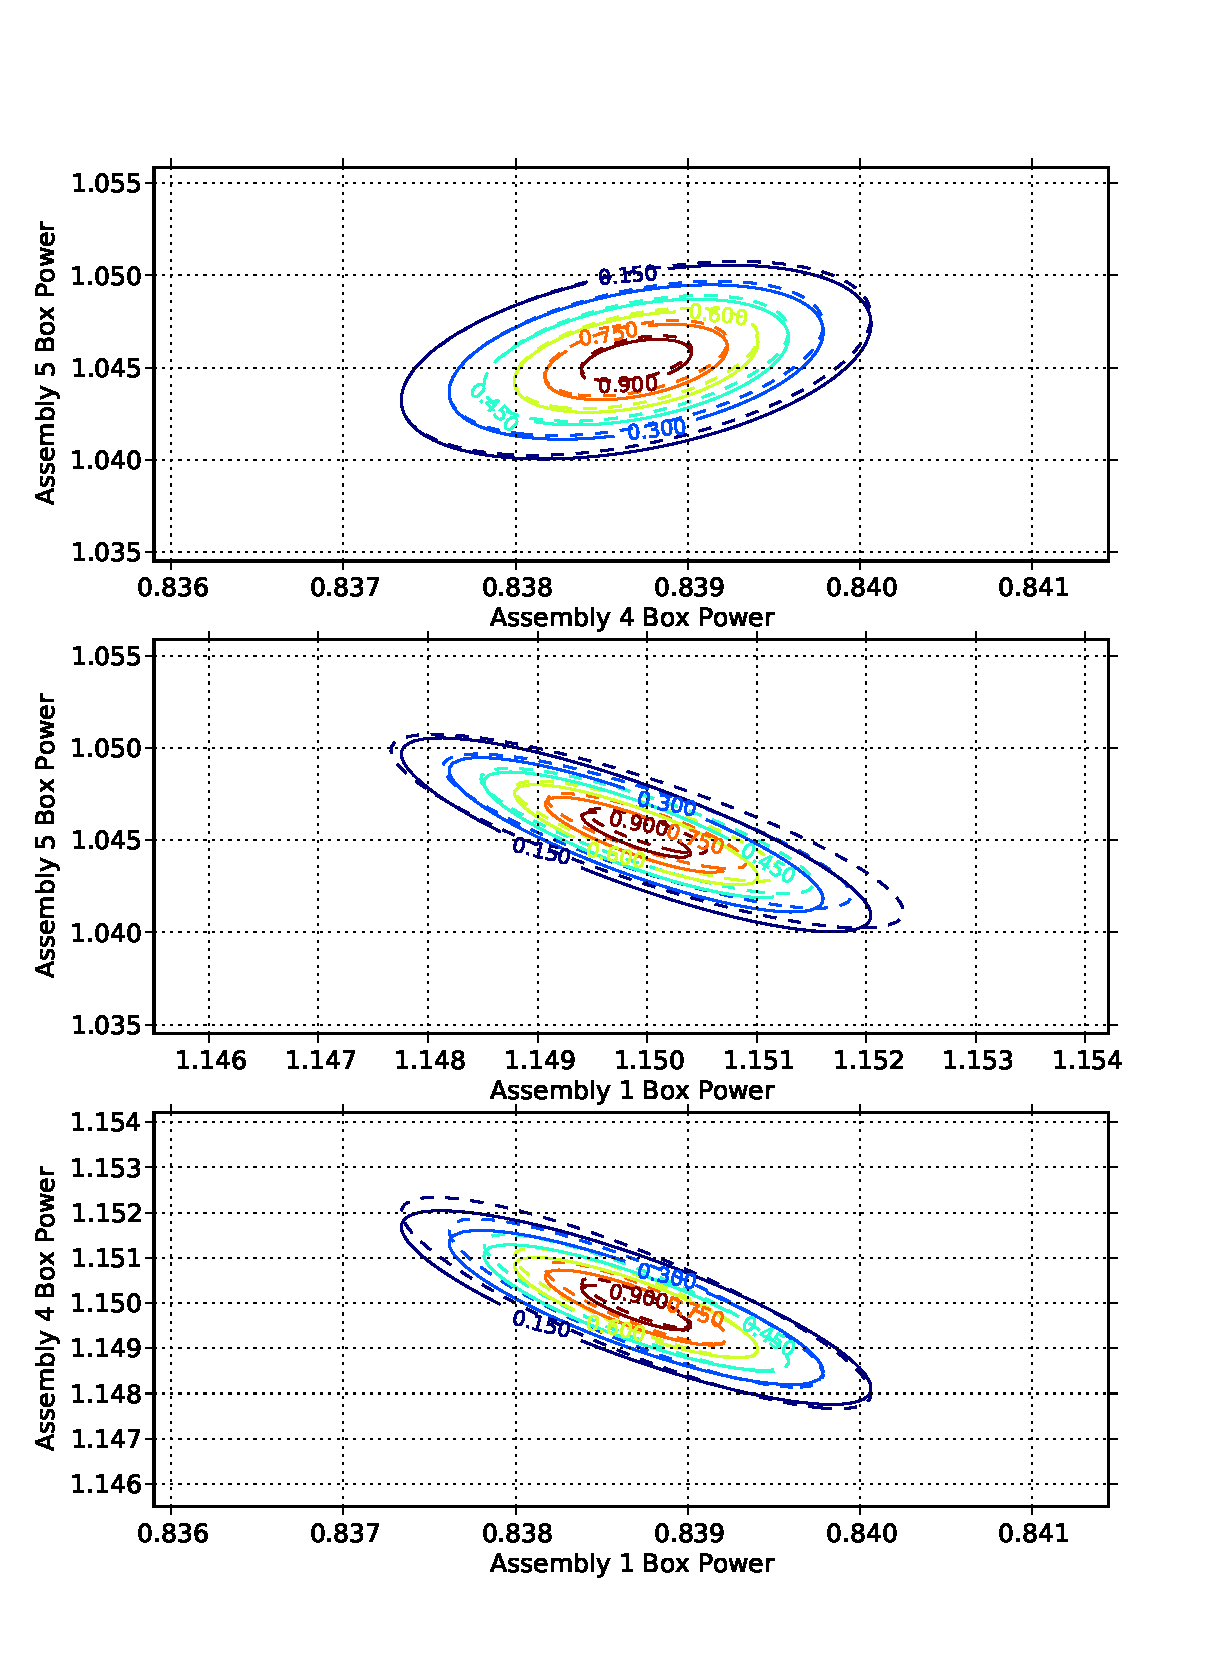
\includegraphics[scale=.70]{./Chapter3/tmi_correlations.pdf}
 \end{center}
\end{figure} 
For each case in Fig. \ref{fig:tmi_correlations} the bivariate distributions are obtained by sampling the reduced order model and \ac{PARCS}. Variations between the overlayed distributions can be attributed to roundoff error. A decrease in the box power of assembly five is equivalent to an increase in the absorption of the assembly's control rods, which effectively shifts the neutron flux away from the central assembly. Consequently, a negative correlation is expected between assemblies one and five and between assemblies one and four. Indeed, statistical sampling has the Pearson correlation coefficient for the box powers of assemblies one and four to be $-0.83$ and $-0.84$ between assemblies one and five. However, negative correlation coefficients between assembly one and assemblies four and five implies a positive correlation coefficient between assemblies four and five. The positive correlation coefficient of $+0.40$ between assemblies four and five is evident in Fig. \ref{fig:tmi_correlations}.  



% General Observations
\section{General Observations}
\label{sec:general_observations}

Before moving on to a large-scale engineering system a few general observations regarding the application of collocation-based and Kriging reduced order models to the uncertainty quantification of the  reactor systems described are in order. Primarily, the demonstration problems indicate that use of only 1D components in the anchored-\ac{ANOVA} expansion provides a very good approximation to the true system under investigation. From a computational point of view, 1D components are cheap to build and their quantity is equal to the number of random variables modeled. Higher order components generally require higher levels of interpolation and so their construction should be minimized if possible. As mentioned in \cite{AHSGC_HighDimensions}, the interaction effects between random variables for most realistic physical systems have a negligible effect on outputs of interest. 

Nevertheless, if multivariate components are needed algorithm \ref{code:rom_algorithm} is able to identify the combination of components most likely to affect the output, which offers significant computational savings. For example, if all components of two random variables were to be included in the anchored-\ac{ANOVA} expansion then 4950 two-dimensional sparse grid interpolants would need to be built. However, if only 5 of the 100 variables are deemed "important" by algorithm \ref{code:rom_algorithm} then only 10 two-dimensional sparse grid interpolants will be built. Not to mention, identification of variables that most affect the variability in some computer code output of interest offers insight into the physical system under consideration. It should be reemphasized that components of the anchored-\ac{ANOVA} used to build reduced order models do not represent the order of effects on the output. Even the 1D component functions can model nonlinear behavior as discussed in section \ref{subsec:anchored_anova}. Rather, the multivariate components describe the effect of input variables upon some output when acting together.    

For the demonstration problems investigated in this chapter, the Clenshaw-Curtis collocation abscissas performed significantly better than Gauss-Patterson. The Clenshaw-Curtis knots offered effectively the same convergence rates as Gauss-Patterson with far fewer function evaluations. Not to mention, Clenshaw-Curtis knots are much easier to generate.

The application of Morris' Algorithm for design variable screening was found to be a visually useful tool for dimension reduction. Whether a computational problem has a large number of dimensions or not the results of Morris' Algorithm can be viewed on a two-dimensional plot. Design variables having the greatest influence on an objective output's behavior become instantly recognizable. After identifying each example problem's key design variables, a reduced order model based on surrogate Kriging was constructed. The Kriging models' ability to reproduce statistics calculated used exact and collocation-based models using only twenty or so basis points demonstrated great promise for further applications.       

However, in all of the example problems analyzed in the current chapter the input uncertainties were calculated systematically beforehand and were therefore relatively small. In other words, engineering judgment never had to be applied in order to estimate the uncertainty of some model input parameter. Uncertainty estimates based on engineering judgment are reasonably expected to be significantly greater than those that can be calculated because more information is known about the latter. The introduction of large uncertainty estimates will be expected in the proceeding application, largely due to the fact that the sources of uncertainty are unknown. Such estimates are expected to negatively impact the smooth construction of surrogate models to represent the applications of interest.          


 

